\documentclass[review]{elsarticle}
%\documentclass[review]{elsarticle}

%\documentclass[final,5p,times,twocolumn]{elsarticle}
%\documentclass[final,5p,times,twocolumn]{elsarticle}
\usepackage[labelfont=bf,justification=raggedright]{caption}
\captionsetup[figure]{name=Fig. ,labelsep=period,singlelinecheck=true,skip=5pt}
%\captionsetup[table]{labelsep=newline,font=footnotesize,singlelinecheck=false,skip=5pt}
%reviewc
%final,5p,times,twocolumn
\usepackage{lineno,hyperref}
\usepackage{float}
%\usepackage{cite}
\modulolinenumbers[5]
\journal{Materials and Design}
%%%%%%%%%%%%%%%%%%%%%%%
\begin{document}
\begin{frontmatter}
\title{Effect of Nanovoid on Fracture Process of Two-Phase $\alpha$($\rm TiAl$)+$\gamma$($\rm Ti_3Al$) Alloy}
%\tnotetext[mytitlenote]{*** \href{http://www.ctan.org/tex-archive/macros/latex/contrib/elsarticle}{CTAN}.}
%% Group authors per affiliation:
%\author{Maomao Wang\fnref{myfootnote}}

\address[mymainaddress]{School of Mechanical and Electronical Engineering, Lanzhou University of Technology. Lanzhou 730050, China}
\begin{abstract}
 The fracture processes of nanocrystalline metallic materia is affected by dislocation, nanovoid and other defects. Existing studies of defect evolution in titanium-aluminium alloy cover the case that voids located in single crystals, inside grain in poly crystals and at the grain boundaries.Molecular dynamics simulation was performed to study the evolution of a spherical nanovoid in $\alpha$+$\gamma$ two-phase titanium-aluminium alloy under uniaxial tension.
\end{abstract}
\begin{keyword}
$\alpha$+$\gamma$ two phase TiAl alloy; void; molecular dynamics
\end{keyword}
\end{frontmatter}
\linenumbers

\section{Introduction}
TiAl alloy has been used as structural material in aviation industry because its inherent advantages such as low density and self-diffusion rates, high elastic module and high strength \cite{Xiong2015}. However, single phase $\gamma-\rm TiAl$ generally brittle at room temperatures and this limits their use in many other fields.Two-phase titanium aluminum alloys with proper phase distribution and grain size exhibit better mechanical performance compared with monolithic constituents $\gamma$(TiAl) and $\gamma$($\rm Ti_3Al$) alloy \cite{intro-structure}.
\begin{figure}
	\centering
	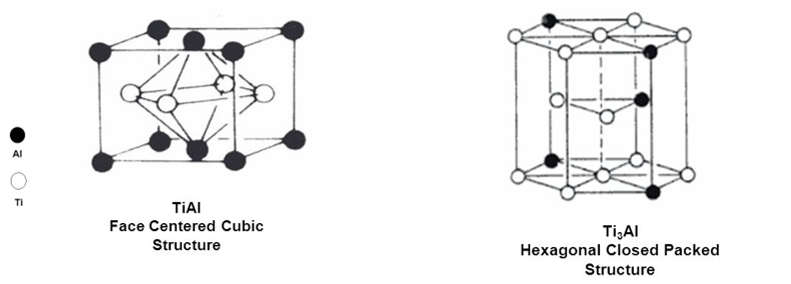
\includegraphics[width=1\linewidth]{img/cell}
	%\label{fig:cell}
	\caption{units cell}
\end{figure}
\subsection{Model creation of nanocrystalline}
$\gamma  TiAl$ has a fcc-centered tetragonal with an $\L1_0$ structure \cite{}, and $\alpha TiAl$ is hcp structure, the structure of the two initial cell are shown in Fig.\cite{}, and the constructing parameters are givin by Table.\cite{}. The simulation cells of two phase poly crystal with an initially spherical void at different position are shown in figure \cite{}. Periodic boundary conditions are applied along all three directions, that makes poly crystal with periodic nanovoid structures. Each cuboidal model, containing about 4.6 million atoms,The initial dimension of simulation cell is  $L_x = nm$, $L_y =  nm$, $L_z =  nm$. The grain orientation and size were randomly created with Voronoi method with code ATOMSK \cite{}, and resulting in the arbitrary shape and orientation of the grains. Only one spherical void defect was placed intragranularlly or intergranularlly within each simulation model void within each simulation model. The intragranular spherical void was located in grain interior of the largest grain of the simulation model, as shown in Fig. \cite{}. The intergranular spherical void was at the center of the simulation cell, as shown in Fig. \cite{}.
\begin{figure}
	\centering
	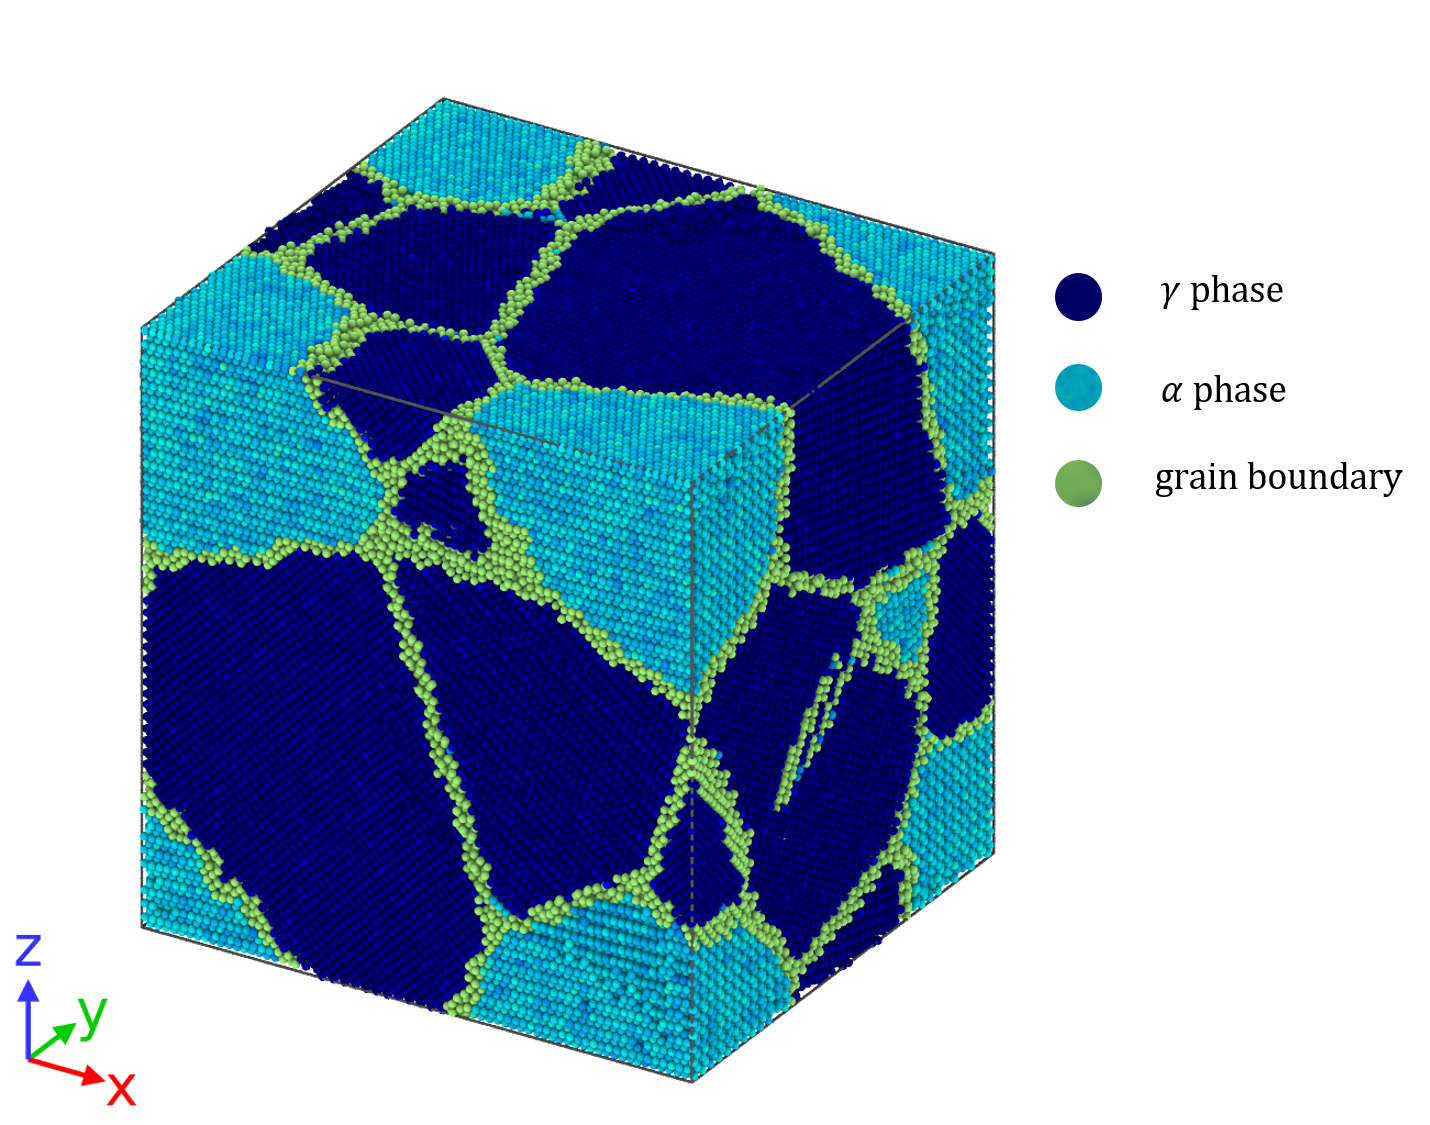
\includegraphics[width=0.7\linewidth]{img/pf_model_labeled}
	\caption{Simulation box}

	%\label{Simulation box}
\end{figure}

\subsection{Atomic potential}
The interaction of particle in the material is determined by interatomic potential. Many reported examples of crack propagation in metal materials were performed with embedded atomic method, due to is better accuracy in metal lattice compare with F-S and L/J \cite{compare LJ and other}. The embedded atom method (MEAM) potential developed by Zope and Mishin by \cite{} was used in the study, which is submitted by MD simulations with the Large-scale Atomic/Molecular Massively Parallel Simulator (LAMMPS) open-source code \cite{}. We performed constant-pressure and constant-temperature(NPT) molecular dynamics simulation.

\subsection{data Analysis method}
\paragraph{Cen}
In view of the fact that dislocations cannot be easily spotted in a three-dimensional crystal, a centrosymmetry parameter \cite{C.L. Kelchner1998} is used to identify the nucleation and propagation of dislocations. The said centrosymmetry parameter is defined as follow:
$$P = \displaystyle\sum_{i=1}^{6}|\vec{R_i}+\vec{R_{i+6}}|^2$$
where $\vec{R_i}$ and $\vec{R_{i+6}}$ are the vectors corresponding to the six pairs of opposite nearest neighbors in the fcc lattice. The centrosymmetry parameter is zero for atoms in a perfect lattice. In other words, if the lattice is distorted the value of P will not be zero. Instead, the parameter will have a value within the range corresponding to a particular defect. By removing all the perfect and surface atoms within the bulk, the existence of dislocation atoms become visible.<Details>
\paragraph{stress}
The atomic stress is calculated using the virial definition :
$$\sigma_t(i)=-$$
$$\sigma_t(i)= $$
\section{Molecular dynamics simulation}


\begin{figure}
	\centering
	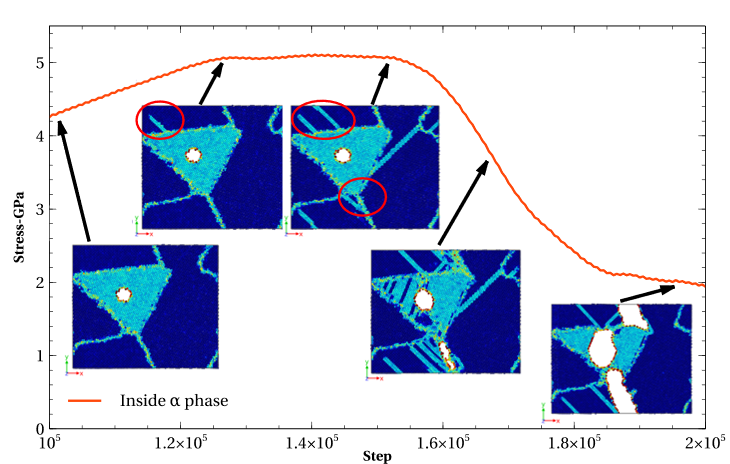
\includegraphics[width=1\linewidth]{img/process-ia}
	\label{fig:process.ia}
	\caption{Fracture process of specimem with void in $\alpha$ pahse}
\end{figure}

\section{Results and Discussion}
\subsection{The influence of void on strength of TiAl alloy}
The existence of void detract the strength, and the void inside $\alpha$ phase grain have most significant  impact on the strength, however the void on the grain boundary have little impact on incipient strength of the material. Detailed observation of specimen with void inside the grain is shown in Figure ~\cite{fig:processia}.
1.In many cases the orientation of slip slip is changed because the crystallographically available slip and directions are not continuous across the interface. This may significantly reduce the Schmid factor and thus impede slip transfer. At the $\gamma/\gamma$ interfaces the orientation of the slip plan could change through a relevantly large angle of about 90 degree. Reorientation of slip is always required at the $\alpha_{2} / \gamma$ interface; the smallest angle between the corresponding slip planes ${1 1 1 }_{\gamma}$ and ${ 1 0 -1 0}_{\alpha_2}$ is about 19 degree ref{}.
2. The core of  a dislocation intersecting an interface often needs to be transformed. For example, an ordinary 1/2<110] dislocation gliding in one $\gamma$ grain has to be converted in to a <101] super dislocation with the double Burgers vector gliding in an adjacent $\gamma$ grain. At the $\alpha/\gamma$ interface the dislocations existing in the $D0_{19}$ structure have to be transformed into dislocations consistent with the $L1_0$structure. These core transformations are associated with a change of the dislocation line energy because the lengths of the Burgers vectors and the shear module are different.
3.Dislocations crossing semi-coherent boundaries have to intersect the misfit dislocations, a process that involves elastic interaction, jog formation and the incorporation of gliding dislocations into the mismatch structure of the interface.When the slip is forced to cross $\alpha_2$ lamellae, pyramidal slip of the $\alpha_2$ phase is required, which needs an extremely high shear stress.


\subsection{Decrease of Strength}
\section{Conclusion}

\bibliographystyle{elsarticle-num.bst}
\section*{References}
\bibliography{/ref/VIOLET-ref}
%Fig.\cite{fig:stress}.
\end{document}
